\section{Rolling Road}
Text

\subsection{BDD}
The Block Definition Diagram in \ref{fig:RR_BDD} gives a general overview of which parts the system is built up by.

\begin{figure}[H]
	\centering
	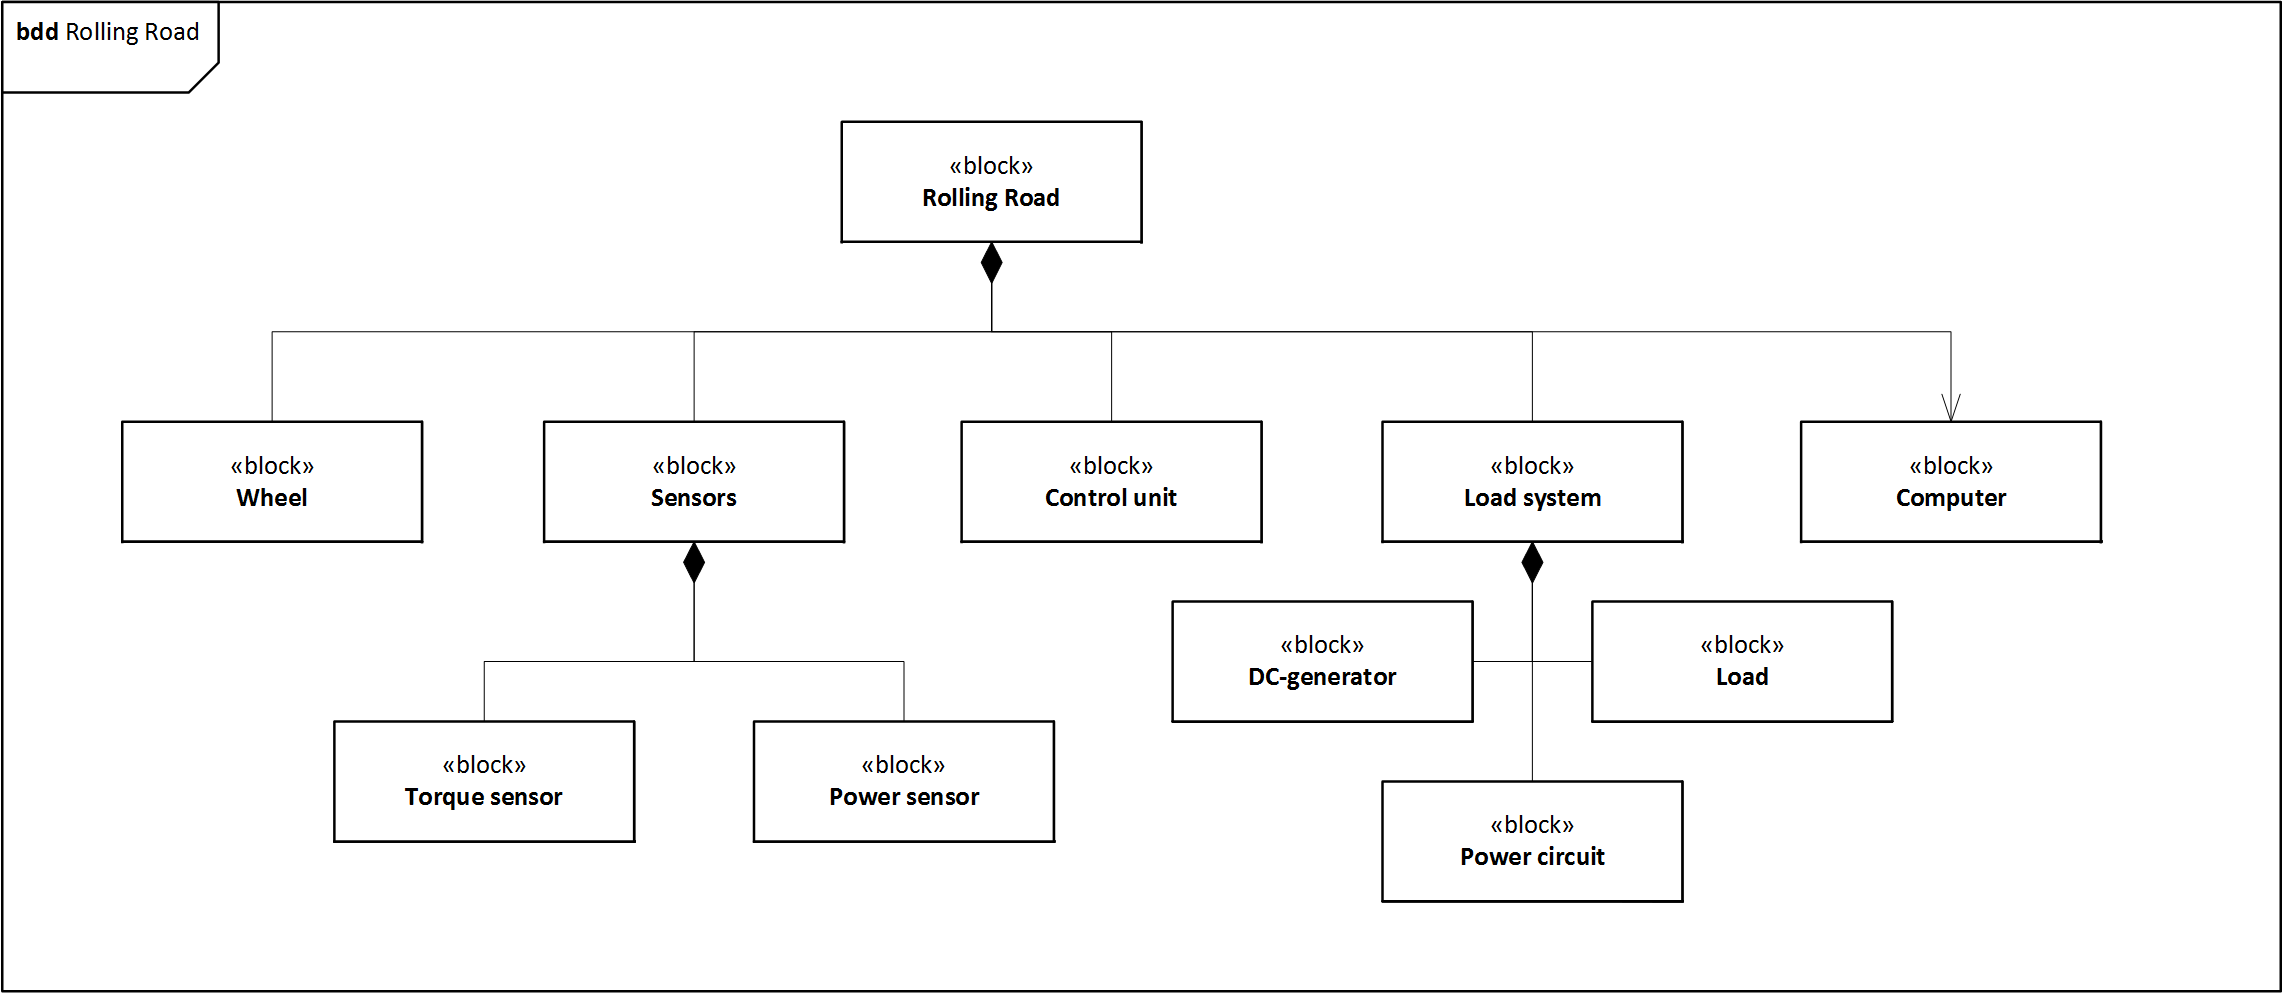
\includegraphics[width=0.9\linewidth]{Architecture/BDD_RollingRoad}
	\caption{BDD for Rolling Road}
	\label{fig:RR_BDD}
\end{figure}

\subsection{IBD}
The Internal Block Diagram in \ref{fig:RR_IBD} gives a general overview of the internal and external communication between the blocks in the system.

\begin{figure}[H]
	\centering
	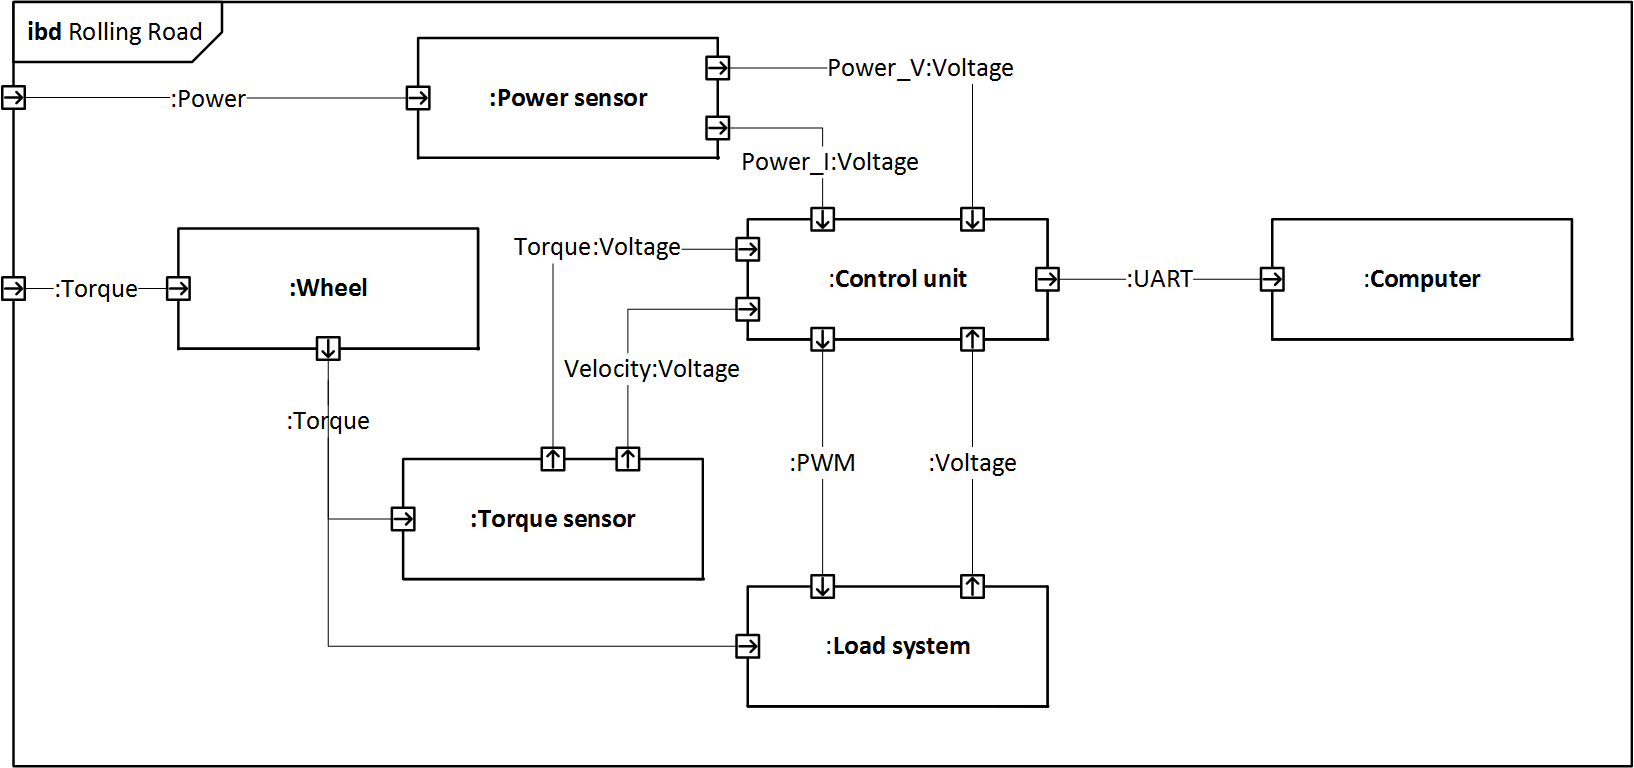
\includegraphics[width=0.9\linewidth]{Architecture/IBD_RollingRoad}
	\caption{IBD for Rolling Road}
	\label{fig:RR_IBD}
\end{figure}

\subsection{Protocol description}
The signals and protocols used to communicate between the blocks in Rolling Road are specified in this section.

\textbf{Block :Power Sensor}\\
The Power sensor receives power from the external power source (battery). Signals representing the voltage and current emit from the Power sensor as voltage 0-5V.\\
Block interface description:

\begin{itemize}
	\item \textbf{:Power}\\
		Direction: [External power source] $\rightarrow$ [Power sensor]\\
		Description: The power received from the external power source.
	\item \textbf{Power\_V :Power}\\
		Direction: [Power Sensor] $\rightarrow$ [Control unit]\\
		Description: An analog signal in the interval 0-5V, which represents the voltage of the power received from the external power source.
	\item \textbf{Power\_I: Voltage}\\
		Direction: [Power Sensor] $\rightarrow$ [Control Unit]\\
		Description: An XXX\fxnote{uddyb signalbeskrivelse} signal in the interval 0-5V, which represents the current of the power received from the external power source.
\end{itemize}

\textbf{Block :Wheel}\\
After:Torque from the Rolling Road wheel, Wheel, represents the Before:Torque from the external car. 
Block interface description:

\begin{itemize}
	\item \textbf{Torque\_In :Torque}\\
		Direction: [External car wheel] $\rightarrow$ [Wheel]\\
		Description: Torque from the car's wheel is transmitted into the system.
	\item \textbf{Torque\_Out :Torque}\\
		Direction: [Wheel] $\rightarrow$ [Torque sensor]\\
		Description: The torque from the system's Wheel goes through a drive-shaft to the Torque sensor.
\end{itemize}

\textbf{Block :Torque sensor}\\
Torque from the Rolling Road wheel, Wheel, goes into the Torque sensor and the Torque sensor transmits two analog Voltage signals that represents the Torque and the Velocity.\\Block interface description:

\begin{itemize}
	\item \textbf{Velocity :Voltage}\\
		Direction: [Torque sensor] $\rightarrow$ [Control Unit]\\
		Description:An analog signal in the interval 0-5V, which represents the angular velocity of the Wheel.
	\item \textbf{Torque :Voltage}\\
		Direction: [Torque sensor] $\rightarrow$ [Control Unit]\\
		Description: An analog signal in the interval 0-5V, which represents the torque from the car through the Wheel.
\end{itemize}

\textbf{Block :Load System}\\
Torque from the Rolling Road wheel, Wheel, goes into the Load system. The Load system receives, from the Control unit, a digital signal, which controls the Load system, and the Load system transmits a Voltage, which represents the current in the Load system to the Control unit.\\
Block interface description:

\begin{itemize}
	\item \textbf{:Torque}\\
		Direction: [Wheel] $\rightarrow$ [Load system]\\
		Description: The Torque of Wheel goes into the Load system.
	\item \textbf{:PWM}\\
		Direction: [Control unit] $\rightarrow$ [Load system]\\
		Description: A digital signal 0V/5V, which controls the Load system.
	\item \textbf{:Voltage}\\
		Direction: [Load System] $\rightarrow$ [Control unit]\\
		Description: An analog signal in the interval 0-5V, which represents the current in the Load system.
\end{itemize}

\textbf{Block :Computer}\\
The Computer receives data from the Control unit via an UART connection.\\
Block interface description:

\begin{itemize}
	\item \textbf{:UART}\\
		Direction: [Control Unit] $\rightarrow$ [Computer]\\
		Description: UART connection to transmit data from Control unit to Computer.
\end{itemize}

\textbf{Block :Control unit}\\
The Control Unit receives analog voltage signals from the Power Sensor that represents the voltage and current of the power from the external power source. The Control Unit also receives analog voltage signals from the Torque Sensor that represents the torque and angular velocity of the torque of the Wheel. The Control Unit controls the Load System with a digital signal and receives an analog signal that represents the current through the Load System. The Control Unit transmits data to the Computer via an UART connection.\\
Block interface description:

\begin{itemize}
	\item \textbf{Power\_V :Voltage}\\
		Direction: [Power Sensor] $\rightarrow$ [Control Unit]\\
		Description: An analog signal in the interval 0-5V, which represents the voltage of the power received from the external power source.
	\item \textbf{Power\_I :Voltage}\\
		Direction: [Power Sensor] $\rightarrow$ [Control Unit]\\
		Description: An XXX \fxnote{uddyb signalbeskrivelse} signal in the interval 0-5V, which represents the current of the power received from the external power source.
	\item \textbf{Velocity :Voltage}\\
		Direction: [Torque Sensor] $\rightarrow$ [Control Unit]\\
		Description: An analog signal in the interval 0-5V, which represents the rotational velocity of the Wheel.
	\item \textbf{Torque :Voltage}\\
		Direction: [Torque Sensor] $\rightarrow$ [Control uUit]\\
		Description: An analog signal in the interval 0-5V, which represents the torque from the car through the Wheel.
	\item \textbf{:PWM}\\
		Direction: [Control Unit] $\rightarrow$ [Load System]\\
		Description: A digital signal 0V/5V, which controls the Load system.
	\item \textbf{:Voltage}\\
		Direction: [Load System] $\rightarrow$ [Control Unit]\\
		Description: An analog signal in the interval 0-5V, which represents the current in the Load system.
	\item \textbf{:UART}\\
		Direction: [Control Unit] $\rightarrow$ [Computer]\\
		Description: UART connection to transmit data from Control unit to Computer.
\end{itemize}